\begin{block}{6. Generation pipeline}
\begin{enumerate}
  \item \textbf{Prompt construction:} Alpaca task + router prompt. Copy exact wrapper signature, then choose: PyTorch fallback, module-level \texttt{torch.compile}, or Triton fusion.
  \item \textbf{Constrained decoding:} Full benchmark results below use one-shot code-block decoding. Separate 6-op EBNF/XGrammar pilot exists, but is excluded from this results table.
  \item \textbf{Compile \& run:} Flex/Bison preflight, then Modal T4. Triton JIT compiles on first call; TritonBench supplies shapes/test inputs.
  \item \textbf{Feedback loop:} No agentic retries during final runs. Failures were converted offline into prompt iterations P8--P12.
\end{enumerate}
\end{block}

\begin{exampleblock}{7. Experimental setup}
\begin{itemize}
  \item \textbf{Benchmark:} TritonBench-T, \texttt{simp} tier, 166 tasks.
  \item \textbf{Hardware:} Modal NVIDIA T4, 16 GB VRAM, CC 7.5.
  \item \textbf{Software:} CUDA 12.4.1, Python 3.12, PyTorch 2.5.1, Triton 3.1.0.
  \item \textbf{LLMs:} Qwen/Qwen-Coder for local LM Studio; Haiku/Sonnet for cheap-vs-strong hosted comparison.
  \item \textbf{Decoding:} one sample/task; LM Studio temp 0.1; Claude provider default; no best-of.
  \item \textbf{Timing:} TritonBench per-op ms; report execution accuracy and same-GPU speedup.
  \item \textbf{Statistics:} one archived full run/model; no p-values claimed. Next: 5 runs, median $\pm$ IQR, Wilcoxon $\alpha=0.05$.
\end{itemize}
\end{exampleblock}

\begin{block}{8. Results}
\textbf{Headline result:} Claude Sonnet 4.6 + Prompt 12 solved 159/166 tasks (95.78\%) with 1.23$\times$ same-GPU speedup.

\begin{table}
\centering
\begin{tabular}{l r r r}
\toprule
\textbf{Method} & \textbf{Correctness} & \textbf{Local speedup} & \textbf{p-value} \\
\midrule
Qwen P9 full              & 74.70\% & 1.24$\times$ & --- \\
Qwen P11 full             & 83.73\% & 1.13$\times$ & --- \\
Claude Haiku P12 full     & 81.33\% & 1.10$\times$ & --- \\
Claude Sonnet P12 full    & 95.78\% & 1.23$\times$ & --- \\
\bottomrule
\end{tabular}
\caption{Full TritonBench-T \texttt{simp} runs, n=166. Local speedup compares generated code to PyTorch remeasured on the same Modal T4.}
\end{table}

\begin{figure}
\centering
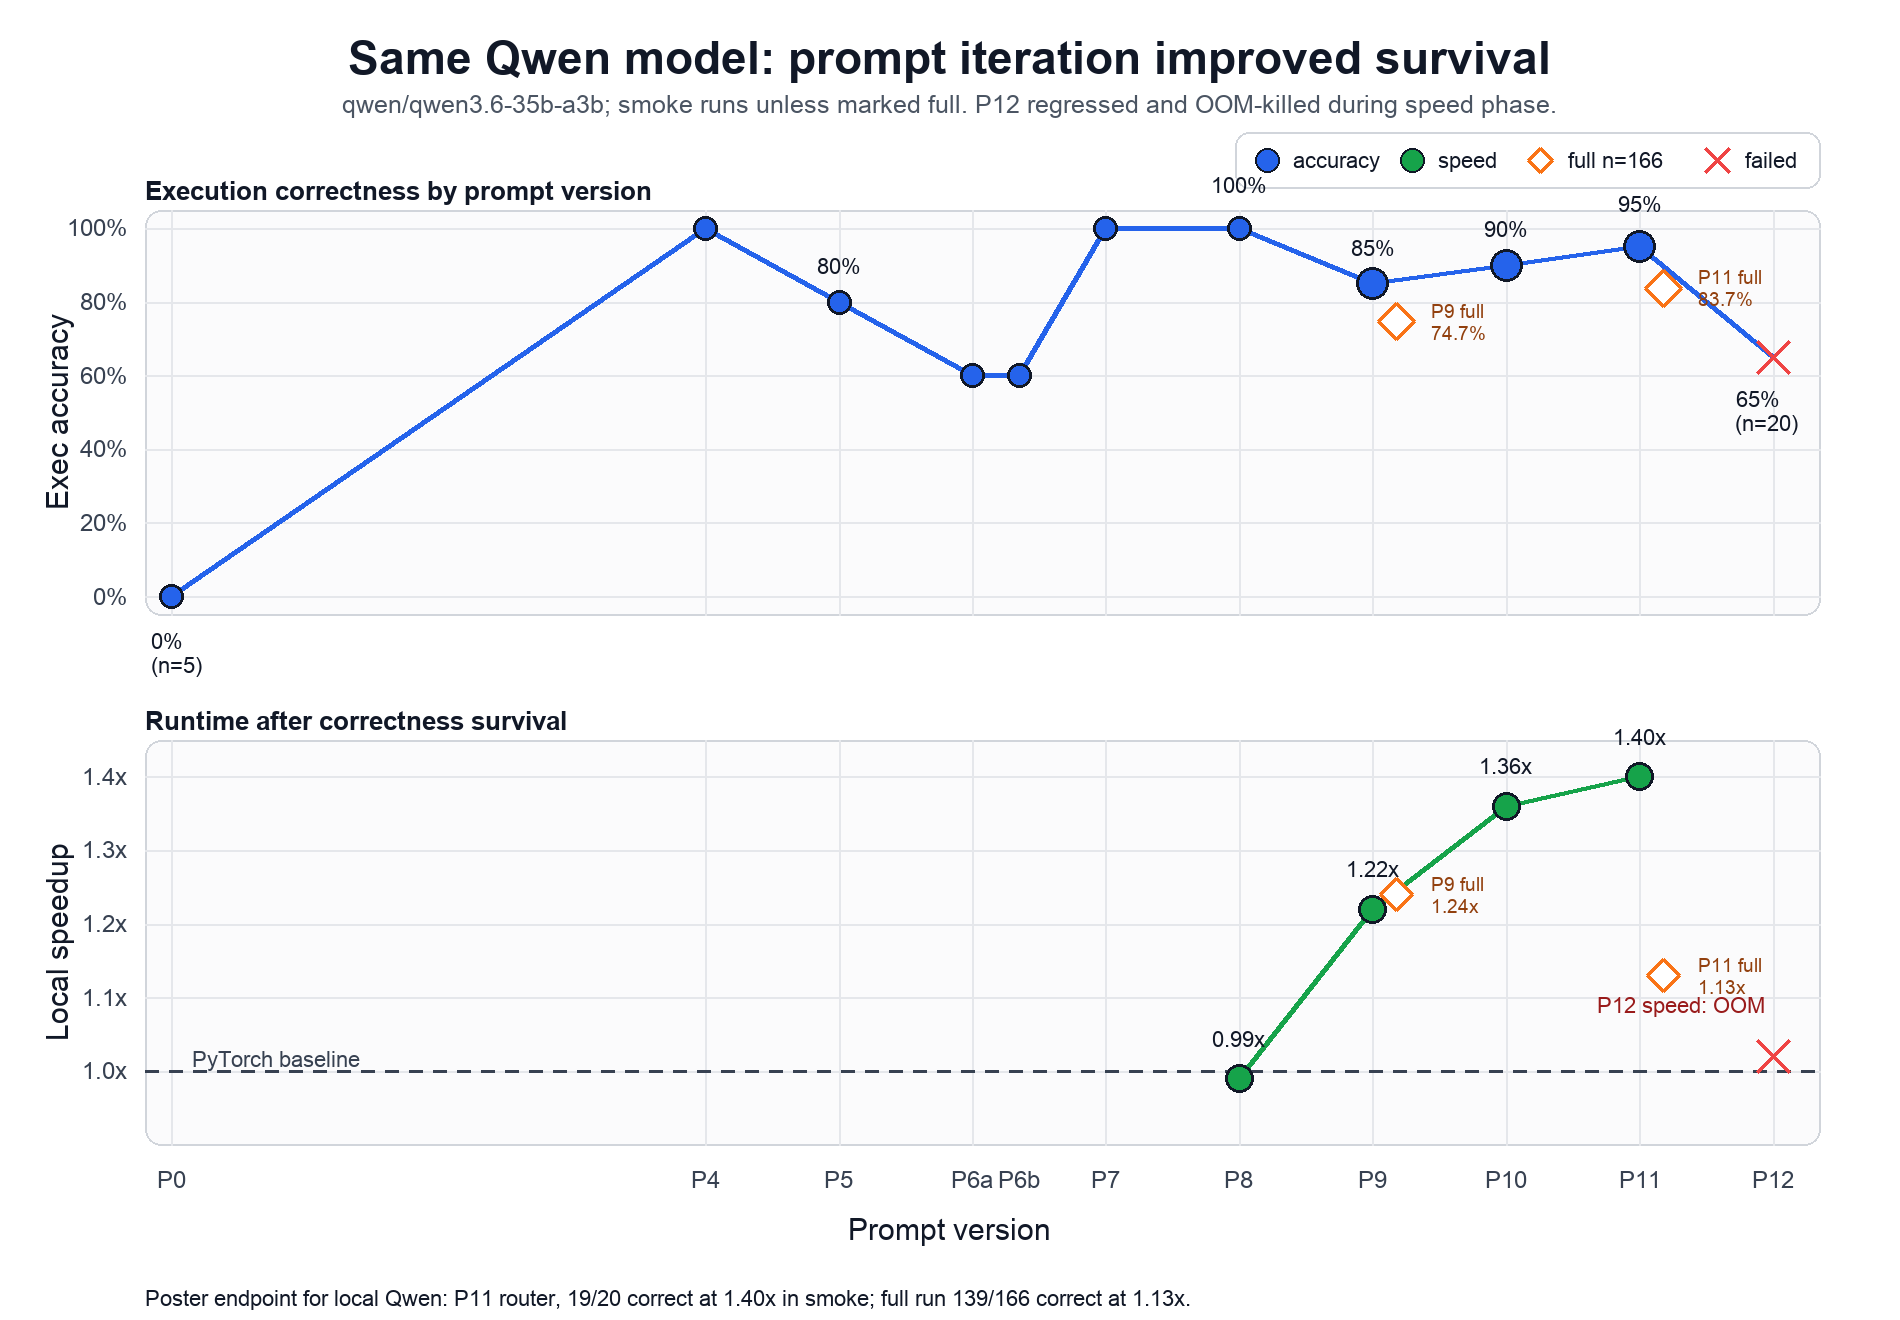
\includegraphics[width=0.85\textwidth]{figures/results_fig.png}
\caption{Correctness-speed tradeoff. Triangles are smoke runs; circles are full 166-task runs.}
\end{figure}
\end{block}

\begin{block}{9. Discussion \& limitations}
\begin{itemize}
  \item \textbf{Wins:} Router prompting made Triton selective, improving full-run survival up to 95.78\%.
  \item \textbf{Failures:} Some families still need semantic checks: optional tensors, signatures, special functions, invalid Triton APIs.
  \item \textbf{Next step:} Add semantic preflight + repeated runs for IQR and Wilcoxon testing.
\end{itemize}
\end{block}

\begin{block}{References}
\nocite{*}
\footnotesize{\bibliographystyle{plain}\bibliography{poster}}
\end{block}
